% SPDX-License-Identifier: CC-BY-SA-4.0
% SPDX-FileCopyrightText: Louis Royer <infos.louis.royer@gmail.com>
\documentclass[../main.tex]{subfiles}
\begin{document}
\initSubfile[4]
% utilisés uniquement pour la compilation isolée du chapitre (à mettre à jour en cas de changement)
\dummylabel{sec:mobility}{1.1.2.5}
\dummylabel{sec:exigences-integration}{2.1}
\dummylabel{sec:migration-copie-a-priori}{2.3.3.2}
\dummylabel{ch:edge-services-integration}{3}
\dummylabel{sec:edge-instance-rebinding}{3.4.2}
\dummylabel{fig:pfcp-one-big-upf}{3.13}
\chapter{Gestion de la mobilité}
\label{ch:mobility}

\begin{chapterHeader}
Ce chapitre est dédié à la gestion de la mobilité et son intégration dans l’architecture~SR4MEC.
Nous détaillons comment la mobilité est effectuée dans les réseaux~5G existants, et exposons les limites de son mécanisme de continuité de service et de session.
Nous présentons des procédures pour prendre en compte les \gl{handover}{\textit{handovers}} dans notre architecture, toujours de manière compatible avec les réseaux~5G existants.
Nous montrons que notre architecture permet de préserver la \gl{SSC}{continuité de la session} des \gl{user}{utilisateurs}, sans compromis sur l’optimalité des chemins vers les \gl{edge}{\textit{edges}}.
\end{chapterHeader}

\section{Problématique}
Dans ce chapitre nous nous intéressons à la mobilité des \gl{user}{utilisateurs}.
Nous avons détaillé dans le \hyperref[ch:edge-services-integration]{chapitre précédent} notre architecture~SR4MEC qui permet d’intégrer des \gl{service/instances}{services}~\textit{edge} dans des réseaux~5G existants.
Nous avons considéré dans un premier temps un réseau où les \gl{user}{utilisateurs} étaient pratiquement statiques, et avons montré que notre architecture satisfaisait à toutes nos autres exigences d’intégrations.

La gestion de la mobilité est une composante fondamentale des réseaux~5G, qui est donc indispensable pour notre architecture.
Nos exigences d’intégration restent identiques à celles définies dans la \hyperref[sec:exigences-integration]{section~\ref*{sec:exigences-integration} du deuxième~chapitre}.
La gestion de la mobilité présente un double enjeu: il faut à la fois préserver la \gl{SSC}{continuité de service et de session}, mais également prendre en compte la mobilité de l’\gl{user}{utilisateur} pour pouvoir éventuellement proposer un changement d’\gl{service/instances}{instance} qui permettra d’améliorer la \gl{QoE}{qualité d’expérience} (voir figure~\ref{fig:mobility}).
Ce changement d’\gl{service/instances}{instance} peut soit être effectué après le \gl{handover}{\textit{handover}}, soit en mettant immédiatement à jour l’\gl{service/instances}{instance} utilisée. Lorsque le \gl{handover}{\textit{handover}} a été anticipé, et que la migration de données entre les \gl{edge}{\textit{edges}} utilise une stratégie de copie \textit{a priori} (voir~section~\ref{sec:migration-copie-a-priori}), cette deuxième option permet d’éviter les dégradations temporaires de la \gl{QoS}{qualité de service}.

Nous décrirons d’abord en détails comment la mobilité est effectuée dans les réseaux~5G existants, et exposerons les limites de son mécanisme de \gl{SSC}{continuité de service et de session}.
Puis nous présenterons des procédures pour intégrer la gestion de la mobilité dans notre architecture~SR4MEC, et l’impact de cette gestion sur le \gl{CUPS}{plan de contrôle}.

\begin{figure}[h]
    \centering
    \includegraphics[width=0.75\linewidth]{14_mobility/figs/mobility.drawio.pdf}
    \captionsetup{singlelinecheck=off}
    \caption[]{Lorsqu’un \gl{user}{utilisateur} se déplace, son \gl{UE}{équipement (UE)} va successivement utiliser différentes \gl{gNB}{gNBs} pour accéder au \gl{service/instances}{service} $\Delta$. Suivant la politique~\textit{edge}, l’\gl{service/instances}{instance} avec laquelle l’\gl{UE}{UE} est en relation peut dépendre de sa localisation au sein du réseau.
    
    La procédure de \textit{handover} doit s’adapter aux différentes situations:
    \begin{itemize}
        \item mobilité \textit{intra-area}~($t=1$) ou \textit{inter-areas}~($t=2$~et~$t=3$);
        \item préservation de l’\gl{service/instances}{instance}~($t=1$~et~$t=2$) ou changement immédiat d’\gl{service/instances}{instance}~($t=3$).
    \end{itemize}
    }
    \label{fig:mobility}
\end{figure}

\pagebreak
\section{Mobilité en 5G}
\label{sec:mobility-in-5G}
Comme présenté dans la \hyperref[sec:mobility]{section~\ref*{sec:mobility} du premier chapitre}, le \gl{handover}{\textit{handover}} désigne l’opération de changement de \gl{BS}{station de base}.
Cette opération peut être initiée par le \gl{CN}{cœur de réseau}, ou par la \gl{gNB}{gNB} sur la base de mesures périodiques de la qualité du signal.

Dans le standard~5G, chaque \gl{PDU Session}{session~PDU} est liée à un \gl{PSA}{\textit{PDU Session Anchor} (PSA)} qui permet d’accéder au réseau de données central.
Dans notre architecture SR4MEC, les \gl{PDU Session}{sessions~PDU} sont également liées à un \gl{PSA}{PSA}, mais accèdent également à plusieurs \gl{edge}{réseaux \textit{edge}}.
Lorsqu’un \gl{handover}{\textit{handover}} est effectué, le nœud utilisé comme~\gl{PSA}{PSA} peut ne plus être optimal.

Le standard décrit 3~modes de gestion de continuité de service et de session qui permettent de prendre en compte les différents besoins des applications.

Le premier mode consiste à préserver la même \gl{PSA}{PSA} tout le long de la durée de vie de la session.
Ce mode permet à l’\gl{UE}{équipement utilisateur} de conserver son adresse~IP, et donc de maintenir la connectivité avec les \gl{service/instances}{services}.
C’est le seul mode qui doit être obligatoirement supporté par tous les \gl{UE}{équipements utilisateurs}.

Les modes~2~et~3 permettent de changer de \gl{PSA}{PSA} et d’établir une nouvelle \gl{PDU Session}{session~PDU}; ils ne permettent pas une transparence totale du point de vue d’une application de l’équipement utilisateur puisqu’ils impliquent un changement d’adresse~IP de l’équipement.

L’un de ces trois~modes est choisi par le \gl{SMF}{SMF} pour la \gl{PDU Session}{session~PDU} lors de son établissement.

Le changement de \gl{PSA}{PSA} est pertinent lorsque le chemin de données utilisé pour l’accès au réseau~central ne répond plus aux contraintes de \gl{QoS}{qualité de service}.
Lorsque l’usage principal se fait à travers des \gl{edge}{réseaux~\textit{edge}}, on peut se permettre de relâcher les contraintes de \gl{QoS}{qualité de service} pour le réseau~central, et on pourra alors généralement se satisfaire du premier mode.

Dans ce chapitre, nous nous plaçons donc dans un scénario où le premier mode est utilisé.
La méthode d’intégration que nous présentons est néanmoins compatible avec les modes~2 et 3 au prix d’une interruption de la continuité de session avec les services~\textit{edge} causée par le changement d’adresse~IP de l’équipement.

Il existe plusieurs types de \gl{handover}{\textit{handovers}} dans les réseaux~5G~\cite{3GPP.TS.23.502}: le \gl{handover}{\textit{handover}}~Xn et le \gl{handover}{\textit{handover}}~N2.

Le \gl{handover}{\textit{handover}}~Xn utilise l’interface du même nom pour effectuer le \gl{handover}{\textit{handover}} à travers un lien radio entre les \gl{gNB}{gNBs} source et cible.
Ce type de \gl{handover}{\textit{handover}} est initié par le \gl{RAN}{RAN}, et n’est donc disponible que lorsque les \gl{gNB}{gNBs} source et cible sont à portée radio.

Lorsqu’il n’est pas possible d’effectuer un \gl{handover}{\textit{handover}}~Xn, ou que le \gl{CN}{cœur de réseau} doit initier un \gl{handover}{\textit{handover}}, la décision est transmise via l’interface~N2.

Dans ce chapitre nous nous focaliserons sur le \gl{handover}{\textit{handover}}~N2 puisqu’il permet de fonder le \gl{handover}{\textit{handover}} sur des informations en provenance de \gl{NF}{fonctions réseau} du \gl{CUPS}{plan de contrôle}, et qu’il est disponible dans toutes les situations.

\pagebreak
\subsection{Procédure de \textit{handover}~N2}
Dans la procédure de \gl{handover}{\textit{handover}}~N2 représentée sur la figure~\ref{fig:handover-n2-3gpp}, l’\gl{UE}{équipement utilisateur} change d’\textit{area}, ce qui implique que l’entièreté du chemin de données entre l’\gl{UE}{UE} et jusqu’au \gl{PSA}{PSA} est changé.
Pour un \gl{handover}{\textit{handover}} \textit{intra-area}, le principe reste le même à quelques simplifications près.

Pour alléger le diagramme, seuls les \gl{UPF}{UPFs} aux extrémités des chemins sont représentés, mais les autres \gl{UPF}{UPFs} intermédiaires doivent bien entendu également être configurés.
Nous supposons que l’\gl{UE}{UE} n’a établi qu’une seule session~\gl{PDU}{PDU}, et que les sessions~\gl{PFCP}{PFCP} ne sont pas mutualisées entre plusieurs sessions~\gl{PDU}{PDU}.
Pour faciliter la lecture, les changements de flux de données du plan utilisateur sont représentés par des doubles-flèches colorées, sur la même la figure que les messages de contrôles (en noir).

Le standard~5G prévoit également la possibilité pour le \textit{handover}~N2 de remplacer l’\gl{AMF}{AMF} lié à la \gl{PDU Session}{session~PDU}; nous présentons une version simplifiée de cette procédure qui fait abstraction de ces détails en représentant le \gl{CP}{plan de contrôle} comme une seule entité.

Lorsque le \gl{RAN}{RAN} détermine qu’un \gl{handover}{\textit{handover}} est nécessaire, il en informe le \gl{CP}{plan de contrôle~5G} en envoyant un message \texttt{Handover~Required} à l’\gl{AMF}{AMF}.
Le \gl{CP}{plan de contrôle} prépare alors un nouveau chemin pour les données utilisateur, qui ne sera utilisé qu’à partir de la synchronisation de l’\gl{UE}{UE} avec la \gl{gNB}{gNB}~cible.
Pour permettre aux \gl{PDU}{PDUs} du lien descendant d’atteindre leur destination même après le changement de \gl{gNB}{gNB}, des règles de \textit{forwarding} sont créées afin de transférer vers la \gl{gNB}{gNB}~cible celles reçues par la \gl{gNB}{gNB}~source.
Suivant la topologie du réseau entre les \gl{gNB}{gNBs} source et cible, le choix sera fait entre un \textit{forwarding}~direct (les \gl{PDU}{PDUs} du lien descendant sont transférées par la \gl{gNB}{gNB}~source directement vers la \gl{gNB}{gNB}~cible en utilisant leur interface~N3) ou indirect (les \gl{PDU}{PDUs} sont d’abord transférées par la \gl{gNB}{gNB}~source vers son \gl{UPF}{UPF\textsubscript{accès}} qui utilise son interface~N9 pour les envoyer dans le nouveau tunnel~\gl{GTP}{GTP} descendant).

Dans le cas du \textit{forwarding}~indirect, l’entièreté du chemin est modifié; il est donc nécessaire d’établir des tunnels~\gl{GTP}{GTP} pour le nouveau lien montant: le \gl{SMF}{SMF} configure de nouvelles sessions~PFCP sur l’ensemble du chemin à l’exception du \gl{PSA}{PSA}, puis l’\gl{AMF}{AMF} envoie un message \texttt{Handover Request} à la \gl{gNB}{gNB}~cible.
Celle-ci alloue des ressources lui permettant d’envoyer et de recevoir du trafic, et informe le plan de contrôle du \gl{TEID}{TEID} alloué au lien descendant pour cette \gl{PDU Session}{session~PDU} grâce à un message \texttt{Handover~Request~Acknowledge}.
La règle~\gl{PFCP}{PFCP} pour le lien descendant est configurée sur l’\gl{UPF}{UPF\textsubscript{accès}}~cible, et une nouvelle session~\gl{PFCP}{PFCP} est établie sur l’\gl{UPF}{UPF\textsubscript{accès}}~source pour permettre le \textit{forwarding} du trafic descendant.

La phase de préparation est alors achevée, et la phase d’exécution commence avec un message \texttt{Handover Command} envoyé par l’\gl{AMF}{AMF} à \gl{gNB}{gNB} source qui lui précise le \gl{TEID}{TEID} à utiliser pour le \textit{forwarding}; la \gl{gNB}{gNB}~source partage une partie des informations reçues avec l’\gl{UE}{UE}, qui est en mesure d’émettre des données sur le lien montant dès qu’il s’est synchronisé avec la \gl{gNB}{gNB}~cible et a confirmé le \gl{handover}{\textit{handover}}~(\texttt{Handover~Confirm}).
Lorsque la \gl{gNB}{gNB} source n’est plus en mesure d’envoyer le trafic utilisateur descendant directement à l’\gl{UE}{UE}, elle renvoie les \gl{PDU}{PDUs} descendantes à l’\gl{UPF}{UPF\textsubscript{accès}}~source en utilisant le \gl{TEID}{TEID} qui a été alloué pour le \textit{forwarding}; les \gl{PDU}{PDUs} sont ensuite renvoyées vers l’\textit{area}~cible.

La \gl{gNB}{gNB}~cible envoie un message \texttt{Handover~Notify} au \gl{CP}{plan de contrôle}, et le \gl{SMF}{SMF} peut alors configurer les règles pour le nouveau chemin du trafic descendant sur l’ensemble des \gl{UPF}{UPFs}, en commençant par l’\gl{UPF}{UPF\textsubscript{accès}} cible et en remontant jusqu’au \gl{PSA}{PSA}.
Les sessions~\gl{PFCP}{PFCP}\textsubscript{source} peuvent être supprimées, ainsi que toutes les ressources dédiées à cette \gl{PDU Session}{session~PDU} sur la \gl{gNB}{gNB}~source.

\enlargethispage{2.5\baselineskip} % pour éviter de se retrouver avec une seule ligne au dessus de la figure
\pagebreak

\begin{figure}[H]
    \centering
    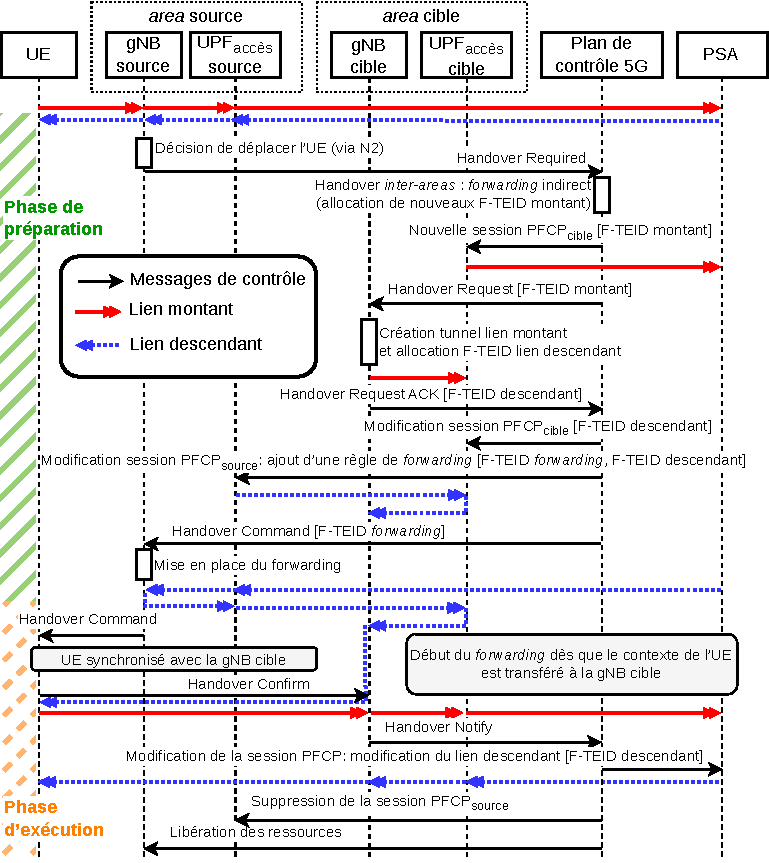
\includegraphics[width=1\linewidth]{figs/handover-n2-3gpp.drawio.pdf}
    \caption[Procédure de \textit{handover}~N2 en 5G]{Procédure de \gl{handover}{\textit{handover}}~N2~\cite{3GPP.TS.23.502}.}
    \label{fig:handover-n2-3gpp}
\end{figure}


\pagebreak
\section{Intégration de la mobilité dans l’architecture proposée SR4MEC}
Dans l’architecture~SR4MEC que nous proposons, notre \textit{Big UPF} joue, du point de vue du \gl{CP}{plan de contrôle~5G}, simultanément le rôle de l’ensemble des \gl{UPF}{UPFs} qui forment le chemin de données.
Il interagit avec le \gl{CP}{plan de contrôle~5G} grâce à son interface commune avec le \gl{SMF}{SMF}.
L’utilisation d’un seul \textit{Big UPF} permet de réduire le nombre de règles~\gl{PFCP}{PFCP} à configurer.
Dans notre modèle les \gl{gNB}{gNBs} sont réparties en plusieurs \textit{areas} qui comprennent chacune une \textit{gateway}~\gl{SR}{SR}, et qui correspond du point de vue du \gl{CP}{plan de contrôle~5G} à une interface~\gl{GTP}{GTP} de notre \textit{Big UPF} (cf.~figure~\ref{fig:integration-mobility}).

\begin{figure}[h]
    \centering
    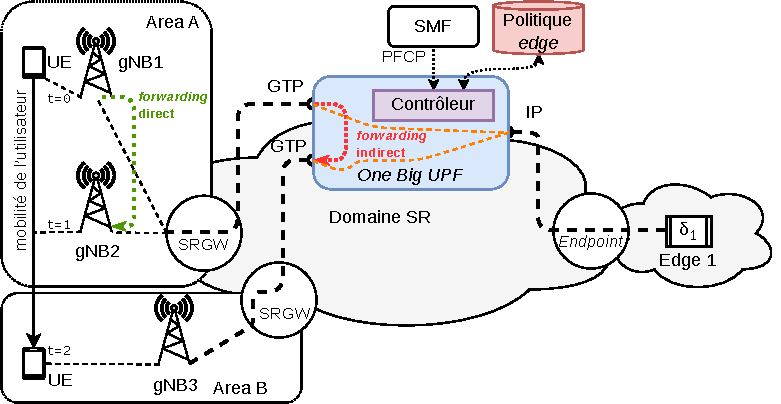
\includegraphics[width=0.75\linewidth]{figs/integration-mobility.drawio.pdf}
    \caption[Gestion de la mobilité avec l’architecture~SR4MEC]{Le \textit{Big UPF} est l’abstraction de l’ensemble des nœuds du domaine~\gl{SR}{SR}; son \gl{controller}{contrôleur} projette les règles~\gl{PFCP}{PFCP} en règles de routage~\gl{SR}{SR}. Dans le cas du \gl{handover}{\textit{handover}}~\textit{intra-area} ($t=1$), le \textit{forwarding} des \gl{PDU}{PDUs} descendantes se fait de manière directe entre les \gl{gNB}{gNBs}~source et cible. Lorsque le \gl{handover}{\textit{handover}} est \textit{inter-areas} ($t=2)$, le \gl{SMF}{SMF} crée une règle~\gl{PFCP}{PFCP} de \textit{forwarding} entre les deux interfaces~\gl{GTP}{GTP} de notre \textit{Big UPF}.}
    \label{fig:integration-mobility}
\end{figure}

Les évènements de mobilité peuvent être pris en compte par la politique~\textit{edge} afin de mettre en relation l’\gl{UE}{équipement utilisateur} avec des \gl{edge}{\textit{edges}} spécifiques.
Comme indiqué dans le tableau~\ref{table:type-proc-mobilite-sr4mec}, nous montrerons dans un premier temps comment effectuer le \gl{handover}{\textit{handover}} en préservant l’\gl{service/instances}{instance}~\textit{edge} utilisée (le changement d’instance pouvant alors être effectué ultérieurement), puis nous montrerons comment mettre à jour l’\gl{service/instances}{instance} directement lors de l’opération de \gl{handover}{\textit{handover}}.

\begin{table}[h]
\center
\begin{tabular}{lll}
\toprule
\thead{Mise en relation} & \thead{Type de mobilité} & \thead{Section} \\
\midrule
Préservation de l’instance & Mobilité au sein d’une \textit{area} (\textit{intra-area}) & Section~\ref{sec:intra-area-mobility} \\
Préservation de l’instance & Mobilité vers une autre \textit{area} (\textit{inter-areas}) & Section~\ref{sec:inter-areas-mobility} \\
Changement immédiat d’instance & Mobilité \textit{intra-area/inter-areas} & Section~\ref{sec:mobility-with-immediate-intance-update} \\
\bottomrule
\end{tabular}
\caption[]{Intégration de la mobilité dans l’architecture proposée~SR4MEC.}
\label{table:type-proc-mobilite-sr4mec}
\end{table}

\pagebreak
\subsection{Mobilité avec préservation de l’instance}
\subsubsection{Mobilité \textit{intra-area}}
\label{sec:intra-area-mobility}
Dans le cas d’une mobilité \textit{intra-area}, nous considérerons que le \textit{forwarding} peut être fait de manière directe entre les \gl{gNB}{gNBs}; la procédure avec le \textit{forwarding}~indirect ne présente pas de différence significative avec une mobilité \textit{inter-areas} qui est traitée dans la section~\ref{sec:inter-areas-mobility}.

Comme nous l’avons observé dans la section~\ref{sec:mobility-in-5G}, les règles émises par le \gl{SMF}{SMF} dépendent de la topologie du réseau entre les \gl{gNB}{gNBs} cible et source, si bien que dans le cas d’une mobilité \textit{intra-area} un seul message \gl{PFCP}{PFCP} est émis par le \gl{SMF}{SMF}.
En effet, puisque l’\textit{area} ne change pas, on peut réutiliser la même règle~\gl{PFCP}{PFCP} pour le lien montant, et il suffit de mettre à jour la règle \gl{PFCP}{PFCP} du lien descendant sur notre \textit{Big UPF}.

La procédure de mobilité \textit{intra-area} dans notre architecture~SR4MEC est illustrée dans la figure~\ref{fig:handover-intra-area}.
La nouvelle règle~\gl{PFCP}{PFCP} configurée par le \gl{SMF}{SMF} contient l’adresse~IP de l’\gl{UE}{UE} ainsi que le \gl{F-TEID}{F-TEID} correspondant au tunnel~\gl{GTP}{GTP} de la \gl{gNB}{gNB}~cible (cf. P1 sur la figure~\ref{fig:handover-intra-area}).
L’intégration de SR4MEC dans ce scénario revient simplement à mettre à jour la règle de routage du lien descendant sur l’\textit{endpoint} en utilisant les informations obtenues en \gl{PFCP}{PFCP}.

\begin{figure}[H]
    \centering
    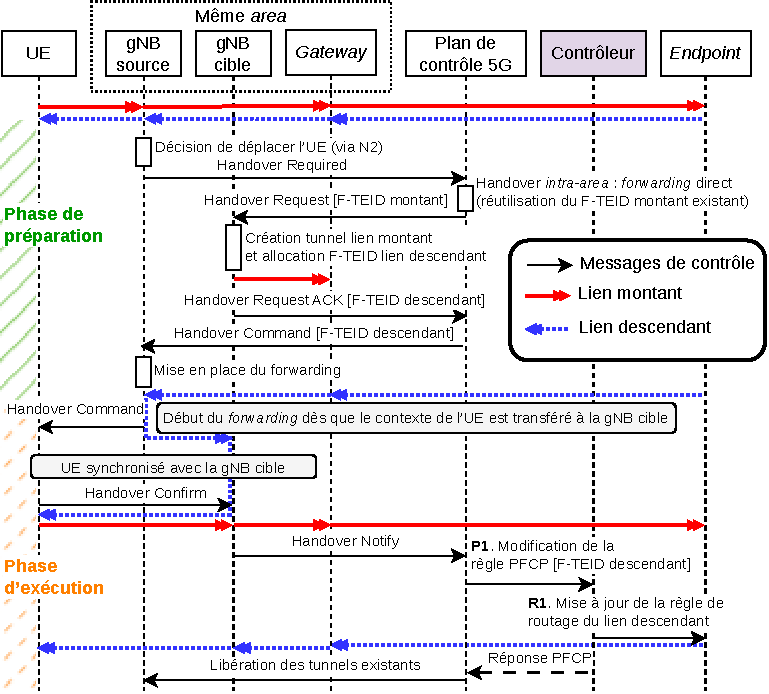
\includegraphics[width=0.8\linewidth]{figs/handover-intra-area.drawio.pdf}
    \caption[Procédure de \textit{handover intra-area} avec SR4MEC]{Intégration de la procédure de \gl{handover}{\textit{handover}} \textit{intra-area} avec notre architecture~SR4MEC.}
    \label{fig:handover-intra-area}
\end{figure}
\pagebreak

\subsubsection{Mobilité \textit{inter-areas}}
\label{sec:inter-areas-mobility}
À la différence du scénario précédent, la mobilité \textit{inter-areas} implique un \textit{forwarding}~indirect puisque les \gl{gNB}{gNBs}~cible et source ne disposent d’un accès direct via leur interface~N3 qu’aux nœuds de la même \textit{area}, ce qui impose le relayage des \gl{PDU}{PDUs} par l’\gl{UPF}{UPF} d’accès (qui correspond dans l’architecture~SR4MEC à la \textit{gateway}~\gl{SR}{SR}).

Les \gl{gNB}{gNBs}~source et cible appartenant à des \textit{areas} différentes, il convient de créer de nouveaux chemins plutôt que de réutiliser ceux existants.
Du point de vue du \gl{SMF}{SMF} les chemins sont créés entre les \gl{gNB}{gNBs} et les interface~\gl{GTP}{GTP} du \textit{Big~UPF}, ce qui réduit le nombre de messages~\gl{PFCP}{PFCP} à échanger.

La procédure de mobilité \textit{inter-area} est schématisée dans la figure~\ref{fig:handover-inter-areas}.
Pendant la phase de préparation du \gl{handover}{\textit{handover}}, le \gl{SMF}{SMF} crée une nouvelle session \gl{PFCP}{PFCP\textsubscript{cible}} sur notre \gl{controller}{contrôleur}~\gl{SR}{SR}.
Une règle~\gl{PFCP}{PFCP} y est configurée pour le lien montant; elle contient l’adresse de l’\gl{UE}{UE}, et utilise l’interface~\gl{GTP}{GTP} correspondant à la \textit{gateway}~\gl{SR}{SR}~cible.
Cette règle~\gl{PFCP}{PFCP} est alors traduite en une règle de routage~\gl{SR}{SR} qui sera créée sur la \textit{gateway}~cible.

Une fois la \gl{gNB}{gNB}~cible configurée, des règles permettant le \textit{forwarding} sont configurées.
Contrairement à toutes les autres règles~\gl{PFCP}{PFCP}, celles permettant le \textit{forwarding} indiquent de créer un lien entre deux interfaces~GTP et non entre une interface~GTP et une interface~IP (cf. pointillés en rouge de la figure~\ref{fig:integration-mobility}).

La session \gl{PFCP}{PFCP\textsubscript{cible}} est d’abord modifiée pour créer un nouveau tunnel~\gl{GTP}{GTP} entre la \textit{gateway}~cible et la \gl{gNB}{gNB}~cible.
Il serait possible de traduire directement cette règle~\gl{PFCP}{PFCP} en règle de routage, mais pour tirer pleinement avantage du routage par segment et économiser la configuration d’une règle, le \gl{controller}{contrôleur} enregistre temporairement les numéros de tunnels sans envoyer de règle de routage aux \textit{gateways}.

La session \gl{PFCP}{PFCP\textsubscript{source}} est ensuite configurée pour créer un nouveau tunnel~\gl{GTP}{GTP} entre les \textit{gateways}~source et cible (\textit{forwarding}).
En utilisant les numéros de tunnels gardés en mémoire ainsi que ceux présents dans la nouvelle règle~\gl{PFCP}{PFCP}, le \gl{controller}{contrôleur} configure une règle de routage~\gl{SR}{SR} sur la \textit{gateway}~source permettant le \textit{forwarding}.

Lorsque l’\gl{UE}{UE} est synchronisé avec la \gl{gNB}{gNB}~cible, la session~PFCP\textsubscript{cible} est modifiée pour remplacer le tunnel de \textit{forwarding} par un nouveau tunnel entre l’interface~IP et l’interface~\gl{GTP}{GTP} de la \textit{gateway}~cible (cf. pointillés en orange de la figure~\ref{fig:integration-mobility}).
Notre \gl{controller}{contrôleur} configure une règle de routage sur la \textit{gateway} grâce aux informations contenues dans la règle~\gl{PFCP}{PFCP}.

La session \gl{PFCP}{PFCP\textsubscript{source}} est désormais inutile et est donc supprimée.
Notre \gl{controller}{contrôleur} peut donc supprimer les règles de routage présentes sur la \textit{gateway}~source.

\pagebreak
\begin{figure}[H]
    \centering
    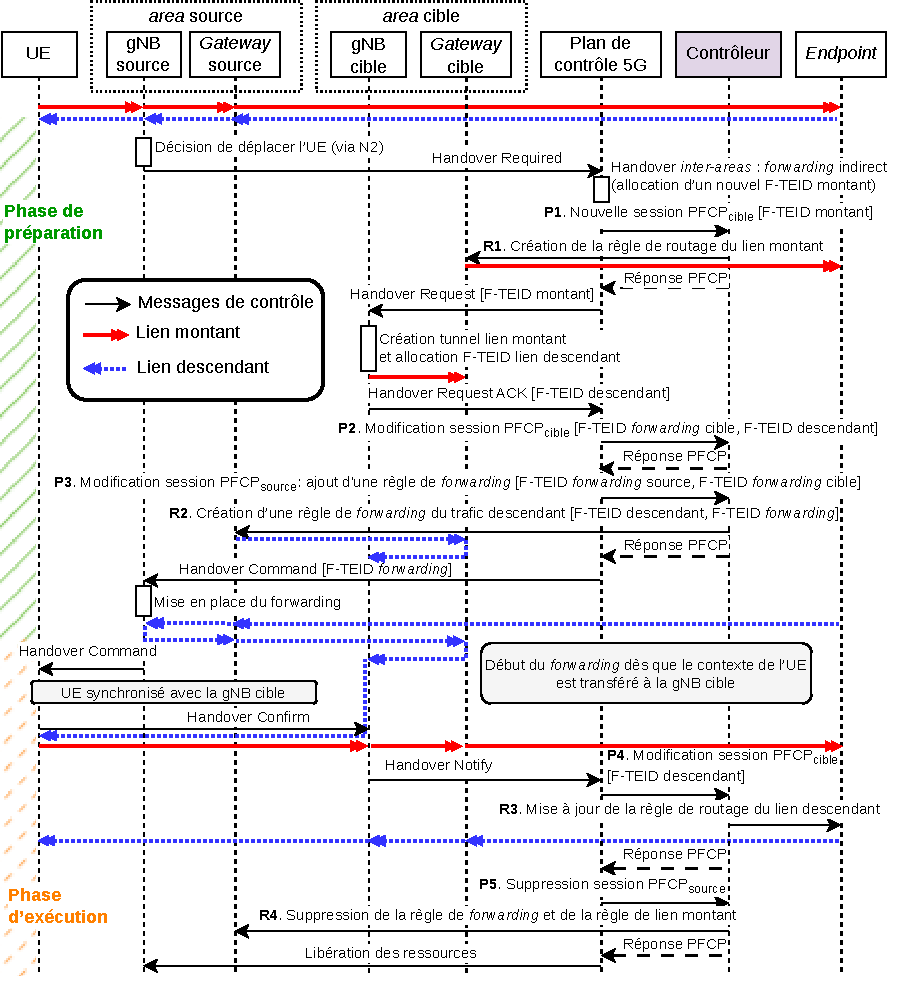
\includegraphics[width=1\linewidth]{figs/handover-inter-areas.drawio.pdf}
    \caption[Procédure de \textit{handover inter-areas} avec SR4MEC]{Intégration de la procédure de \gl{handover}{\textit{handover}} \textit{inter-areas} avec notre architecture~SR4MEC.}
    \label{fig:handover-inter-areas}
\end{figure}

\pagebreak
\subsection{Mobilité avec changement immédiat d’instance}
\label{sec:mobility-with-immediate-intance-update}
Nous avons vu comment s’intègre la procédure de \gl{handover}{\textit{handover}}~N2 lorsque l’on souhaite préserver l’\gl{service/instances}{instance}~\textit{edge}.
Dans nos exigences d’intégration, selon la politique~\textit{edge}, la mobilité d’un utilisateur peut induire un changement d’\gl{service/instances}{instance}.
Une approche naïve consiste à effectuer ce changement \textit{a posteriori}, c’est-à-dire une fois la procédure de \gl{handover}{\textit{handover}} achevée.
Cependant, cette approche implique l’utilisation d’une \gl{service/instances}{instance} moins optimale durant l’intervalle de temps entre la fin de la procédure de \gl{handover}{\textit{handover}} et la fin de la procédure de changement d’\gl{service/instances}{instance}.

En regroupant en une seule procédure le \gl{handover}{\textit{handover}} et le changement d’\gl{service/instances}{instance}, nous pouvons réduire le nombre de règles à configurer.

Dans le cas d’un \gl{handover}{\textit{handover}} \textit{intra-area}, le changement immédiat d’\gl{service/instances}{instance} consiste simplement à remplacer l’opération de mise à jour de la règle de routage du lien descendant par les opérations suivantes:
\begin{enumerate}
    \item Créer une règle de routage pour le lien descendant sur l’\textit{endpoint}~\gl{SR}{SR} de l’\gl{edge}{\textit{edge}}~cible.
    \item Mettre à jour la règle pour le lien montant sur la \textit{gateway}~\gl{SR}{SR} pour diriger le trafic vers l’\gl{edge}{\textit{edge}}~cible.
    \item Après l’écoulement d’un délai suffisant, supprimer la règle de routage pour le lien descendant de l’\gl{edge}{\textit{edge}}~source.
\end{enumerate}

Le scénario \textit{intra-area} étant simple, nous étudions donc le cas plus complexe du \gl{handover}{\textit{handover}} avec changement d’\textit{areas} représenté sur la figure~\ref{fig:handover-inter-areas-new-edge}.

À la différence du scénario de mobilité \textit{inter-areas} avec préservation d’\gl{service/instances}{instance}, lorsque les règles de \textit{forwarding} sont configurées, une règle de routage est également créée sur l’\gl{edge}{\textit{edge}}~cible pour le lien nouveau descendant (cf. R3 sur la figure~\ref{fig:handover-intra-area}).
La création de ce lien descendant entre l’\gl{edge}{\textit{edge}}~cible et la \gl{gNB}{gNB}~cible permet un changement d’\gl{service/instances}{instance} avant la fin de la procédure de \gl{handover}{\textit{handover}}, dès que l’\gl{UE}{équipement utilisateur} est synchronisé avec la \gl{gNB}{gNB}~cible.

Puisque le changement d’\gl{service/instances}{instance} s’effectue conjointement avec le changement d’\gl{edge}{\textit{edge}}, il n’est pas nécessaire de créer un lien montant temporaire vers l’\gl{edge}{\textit{edge}}~source, ce qui économise deux opérations (la création puis la suppression de la règle de routage).
En revanche, puisque les \gl{edge}{\textit{edges}}~source et cible sont deux nœuds~\gl{SR}{SR} différents, la suppression de la règle de routage du lien descendant sur l’\gl{edge}{\textit{edge}}~source n’est plus effectuée simultanément avec la création du nouveau chemin descendant: deux messages de contrôles sont donc nécessaires (notés R3 et R4 sur la figure~\ref{fig:handover-inter-areas-new-edge}).

\pagebreak
\begin{figure}[H]
    \centering
    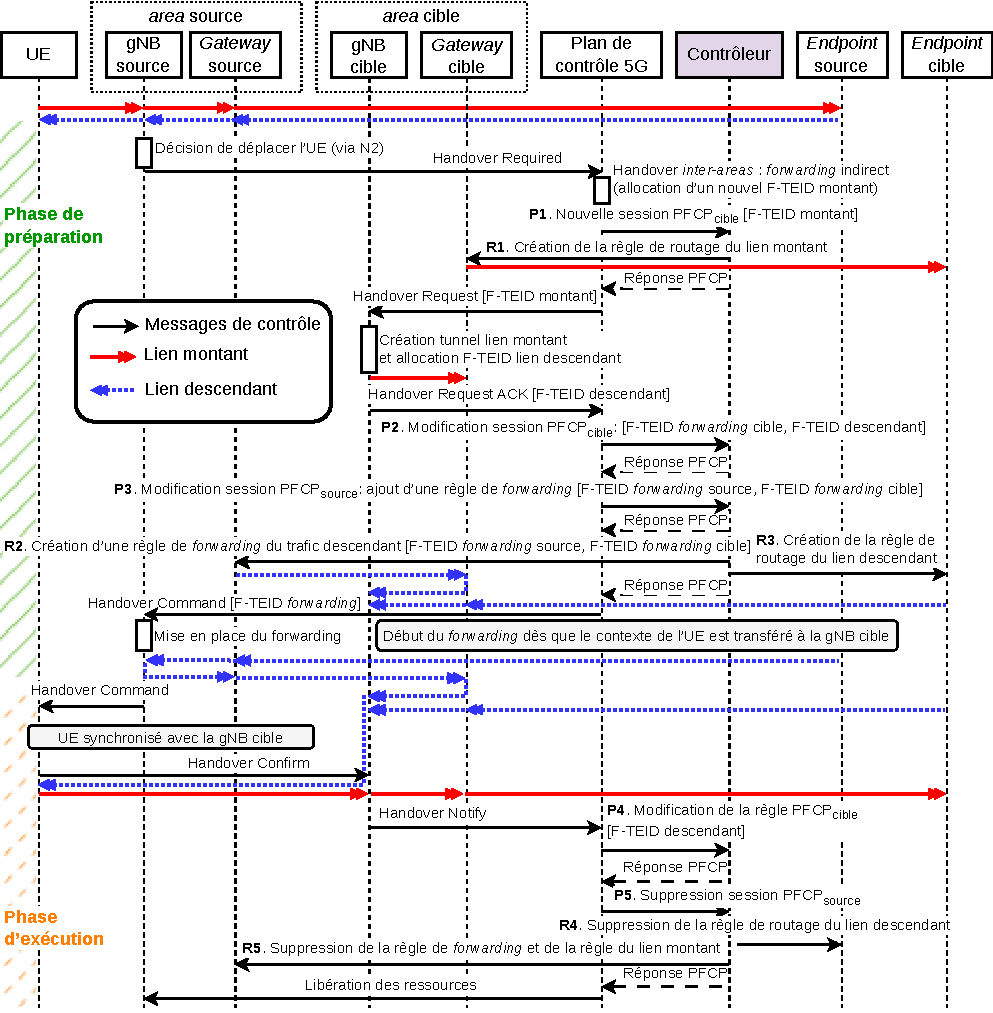
\includegraphics[width=1\linewidth]{figs/handover-inter-areas-new-edge.drawio.pdf}
    \caption[Procédure de \textit{handover inter-areas} avec mise à jour immédiate de l’instance avecSR4MEC]{Mise à jour immédiate de l’\gl{service/instances}{instance}~\textit{edge} lors de la procédure de \textit{handover} \textit{inter-area}.}
    \label{fig:handover-inter-areas-new-edge}
\end{figure}

\pagebreak

\enlargethispage{\baselineskip} % pour éviter une ligne toute seule sous le tableau
\subsection{Impact sur le plan de contrôle}
\label{sec:mobility-impact}

Pour déterminer l’impact de notre architecture sur le \gl{CUPS}{plan de contrôle} lors d’un \gl{handover}{\textit{handover}}~N2, nous comparons le nombre de messages nécessaires dans des scénarios équivalents.

Seuls les scénarios préservant l’\gl{service/instances}{instance} sont décrits par le standard~5G puisqu’il n’intègre pas la notion d’\gl{service/instances}{instance}~\textit{edge}.
Cependant, il est possible d’effectuer un changement d’\gl{service/instances}{instance} soit \textit{a posteriori}, c’est-à-dire en préservant l’\gl{service/instances}{instance} puis en la mettant à jour avec la méthode décrite dans la \hyperref[ch:edge-services-integration]{section~\ref*{sec:edge-instance-rebinding} du chapitre précédent}, soit en adaptant la procédure de \gl{handover}{\textit{handover}}.

Dans le tableau~\ref{table:mobility-impact}, nous exprimons le nombre de messages~\gl{PFCP}{PFCP} échangés en fonction du nombre d’\gl{UPF}{UPFs} intermédiaires que comportent:
\begin{itemize}
    \item le chemin entre les \gl{UPF}{UPFs} de l’\textit{area}~source et l’\gl{edge}{\textit{edge}}~source ($\mathit{UPF_s}$);
    \item le chemin entre les \gl{UPF}{UPFs} de l’\textit{area}~cible et l’\gl{edge}{\textit{edge}}~cible ($\mathit{UPF_c}$);
    \item et l’éventuel chemin de transition entre les \gl{UPF}{UPFs} de l’\textit{area}~cible et l’\gl{edge}{\textit{edge}}~source ($\mathit{UPF_t}$).
\end{itemize}
Nous considérons qu’avec une architecture classique, les chemins comportent au minimum deux \gl{UPF}{UPFs}, situés respectivement dans l’\textit{area} et dans le \gl{edge}{réseau~\textit{edge}}.

Lors de la création ou modification d’un chemin, les \gl{TEID}{TEIDs} sont attribués séquentiellement en commençant par les nœuds situés en sortie du chemin de données; les créations ou modifications de règles~\gl{PFCP}{PFCP} sont donc configurées séparément pour le lien montant et le lien descendant.
Les suppressions de session~\gl{PFCP}{PFCP} sont en revanche comptabilisées comme un unique message~\gl{PFCP}{PFCP} par session.

Par exemple, pour le scénario de préservation de l’\gl{service/instances}{instance} avec une mobilité \textit{inter-areas}, le nombre de messages~\gl{PFCP}{PFCP} requis dans le cas d’une architecture~5G classique est $5 + |\mathit{UPF_s}| + 2 \times |\mathit{UPF_c}|$.
Dans cette formule, nous comptabilisons d’abord 5~messages obligatoires pour
\begin{enumerate*}[label=(P\arabic*), itemjoin={{, }}, itemjoin*={{, et }}]
    \item la création de la session~\gl{PFCP}{PFCP}\textsubscript{cible} sur l’\gl{UPF}{UPF}\textsubscript{accès}~cible
    \item la modification de cette session pour y ajouter une règle de lien descendant
    \item l’ajout d’une règle de \textit{forwarding} sur l’\gl{UPF}{UPF}\textsubscript{accès}~source
    \item la modification de la règle de lien descendant sur le \gl{PSA}{PSA}
    \item la suppression de la session \gl{PFCP}{PFCP}\textsubscript{source} sur l’\gl{UPF}{UPF}\textsubscript{accès}~source.
\end{enumerate*}
Puis nous comptabilisons les messages qui dépendent du nombre de nœuds intermédiaires: la suppression de l’ancien chemin ($|\mathit{UPF_s}|$) ainsi que la création des chemins montant et descendant ($2 \times |\mathit{UPF_c}|$).

\begingroup
\renewcommand{\arraystretch}{1.25}
\begin{table}[ht]
\center
\begin{tabular}{cc|c|cc}
\toprule
\multicolumn{2}{l|}{\thead{Scénario}}                       & \thead{Architecture~5G classique} & \multicolumn{2}{l}{\thead{SR4MEC}}   \\
\thead{Mise en \\ relation}  & \thead{Mobilité} & \thead{Messages~\gl{PFCP}{PFCP}}  & \thead{Messages \\ \gl{PFCP}{PFCP}}    & \thead{Mise à jour \\ des règles~\gl{SR}{SR}} \\
\midrule
\multirow{2}{*}{\makecell{Préservation de \\ l’\gl{service/instances}{instance}}}
    & \textit{intra-area}
        & $1$
        & $1$ & $1$ \\
    & \textit{inter-areas}
        & $
          5 +          |\mathit{UPF_{s}}|
            + 2 \times |\mathit{UPF_{c}}|
          $
        & $5$ & $4$ \\
\midrule
\multirow{2}{*}{\makecell[c]{Changement \\ \textit{a posteriori}}}
    & \textit{intra-area}
        & $
          7 +          |\mathit{UPF_{t}}| % t = temporaire
            + 2 \times |\mathit{UPF_{c}}| % c = cible
          $
        & $1$ & $4$ \\
    & \textit{inter-areas}
        & $
         11 +          |\mathit{UPF_{s}}| % s = source
            + 3 \times |\mathit{UPF_{t}}| % t = temporaire
            + 2 \times |\mathit{UPF_{c}}| % c = cible
         $
        & $5$ & $7$ \\
\midrule
\multirow{2}{*}{\makecell[c]{Changement \\ immédiat}}
    & \textit{intra-area}
        & $
          5 +          |\mathit{UPF_{s}}|  % s = source
            + 2 \times |\mathit{UPF_{c}}|  % c = cible
          $
        & $1$ & $3$ \\
    & \textit{inter-areas}
        & $
          7 +          |\mathit{UPF_{s}}| % s = source
            + 2 \times |\mathit{UPF_{c}}| % c = cible
          $
        & $5$ & $5$ \\
\bottomrule
\end{tabular}
\caption[Impact de SR4MEC sur le plan de contrôle lors de la mobilité]{Comparaison du nombre de messages de contrôle nécessaires pour un \gl{handover}{\textit{handover}}~N2 selon l’architecture utilisée et suivant le scénario.}
\label{table:mobility-impact}
\end{table}
\endgroup

Avec l’architecture classique, seul le cas d’une mobilité \textit{intra-area} avec préservation d’instance est constant puisqu’il nécessite un unique message.
Dans l’architecture~SR4MEC, où le nombre de messages échangés est systématiquement constant, on remarquera que pour tous les autres scénarios le travail du \gl{SMF}{SMF} est considérablement réduit.

Concernant les scénarios avec changement d’\gl{service/instances}{instance} \textit{a posteriori}, une fois le \gl{handover}{\textit{handover}} effectué, la mise à jour de l’\gl{service/instances}{instance} nécessite à elle seule $6 + 2 \times |\mathit{UPF_t}| + |\mathit{UPF_c}|$ messages~\gl{PFCP}{PFCP} supplémentaires avec une architecture~5G classique, alors qu’avec l’architecture~SR4MEC, 3~mises à jour de règles~\gl{SR}{SR} suffisent.
Outres ses avantages en terme de \gl{QoS}{qualité de service}, le changement immédiat d’\gl{service/instances}{instance} réduit largement le nombre de messages~\gl{PFCP}{PFCP} nécessaire pour une architecture~5G classique.
Pour une mobilité~\textit{inter-areas} avec une architecture~5G classique, la procédure ne nécessite que l’ajout que deux messages~\gl{PFCP}{PFCP}: en effet, il faut créer le \gl{TEID}{TEID} du lien montant sur l’\gl{UPF}{UPF} de l’\gl{edge}{\textit{edge}}~cible, et supprimer la session~\gl{PFCP}{PFCP} sur l’\gl{UPF}{UPF} de l’\gl{edge}{\textit{edge}}~source.
Lors d’une mobilité~\textit{intra-area}, ces changements sont compensés par le regroupement des \gl{UPF}{UPFs} de l’\textit{area} et par l’utilisation d’un \textit{forwarding}~direct.

Lorsque l’on utilise notre architecture~SR4MEC, le changement immédiat d’\gl{service/instances}{instance} permet de réduire le nombre de règles~\gl{SR}{SR} à configurer:
\begin{itemize}
    \item Pour la mobilité~\textit{intra-area}, il n’est plus nécessaire de mettre à jour temporairement la règle descendante sur l’\textit{endpoint}~source. Lorsque le \textit{forwarding} se termine, la communication se fait directement avec l’\gl{edge}{\textit{edge}}~cible.
    \item Pour la mobilité~\textit{inter-areas}, il n’est plus nécessaire ni de configurer la \textit{gateway}~source avec une règle vers l’\textit{area}~cible, ni de supprimer cette règle.
\end{itemize}

\section{Synthèse}
Dans ce chapitre, nous avons montré comment intégrer la gestion de la mobilité dans notre architecture~SR4MEC.
Nous avons proposé plusieurs procédures de \gl{handover}{\textit{handover}}, compatibles avec les réseaux~5G existants et s’adaptant au type de mobilité (\textit{intra-area}/\textit{inter-areas}), qui prennent en compte la mise en relation avec des \gl{service/instances}{instances}~\textit{edge}.
Selon la politique~\textit{edge}, il est possible de préserver les relations avec \gl{service/instances}{instances}~\textit{edges} ou de changer d’\gl{service/instances}{instance}.

Nous avons comparé notre architecture~SR4MEC à une architecture~5G classique afin de déterminer son impact sur le \gl{CUPS}{plan de contrôle} dans différents scénarios.
Nous avions montré dans le \hyperref[ch:edge-services-integration]{chapitre précédent} que notre architecture permet de réduire le travail du \gl{SMF}{SMF} pour les établissements de session et les changements d’instance; dans ce chapitre nous avons montré que cette propriété s’applique également aux \gl{handover}{\textit{handovers}}.

Dans ce chapitre et celui qui précède, nous avons étudié le cadre théorique de l’intégration de l’\textit{edge} dans les réseaux~5G.
Nous présenterons dans le prochain chapitre notre plateforme qui implémente notre architecture~SR4MEC et intègre plusieurs implémentations d’\gl{UPF}{UPFs}~5G classiques, et évaluerons notre architecture expérimentalement.
\end{document}